\section{Introduzione}
La specifica della Prova Finale di Reti Logiche 2023/2024 riguarda la progettazione di un modulo hardware che interfacciandosi con una memoria valuti la credibilità dei valori presenti.
\newline
Un esempio pratico potrebbe essere un termometro che registra in memoria la temperatura di una stanza e in caso di dati mancanti il modulo li ricostruisce assegnandogli un adeguato valore di credibilità. Nello specifico, se una misurazione viene ritenuta valida per 5 secondi, allo scadere del lasso di tempo se non è stata memorizzata una nuova misurazione, il modulo decrementa la credibilità dell'ultima temperatura valida fino all'inserimento di un nuovo valore da parte del termometro.

\subsection{Specifica generale}
A livello generale, il sistema legge un messaggio costituito da una sequenza di K parole W il cui valore è compreso tra 0 e 255. La parola "0" all'interno della sequenza sta ad indicare che il valore non è specificato. La sequenza da elaborare è memorizzata a partire da un indirizzo specificato (ADD), ogni 2 byte (i.e. ADD, ADD+2, ADD+4, ..., ADD+2*(K-1)).
\newline
Il modulo da progettare ha il compito di completare la sequenza, sostituendo gli zero laddove presenti con l'ultimo valore letto diverso da zero, ed inserendo un valore di "credibilità" C, nel byte mancante, per ogni valore della sequenza. La sostituzione degli zero avviene copiando l'ultimo valore valido (non zero)
letto precedente e appartenente alla sequenza. Il valore di credibilità C è pari a 31 ogni volta che il valore W della sequenza è non zero, mentre viene decrementato rispetto al valore precedente ogni volta che si incontra uno zero in W. Il valore C associato ad ogni parola W viene memorizzato in memoria nel byte subito successivo (i.e. ADD+1 per W in ADD, ADD+3 per W in ADD+2,...). Il valore C è sempre maggiore o uguale a 0 ed è reinizializzato a 31 ogni volta che si incontra un valore W diverso da zero. Quando C raggiunge il valore 0 non viene ulteriormente decrementato.
\newline

\begin{figure}[H]
    \centering
    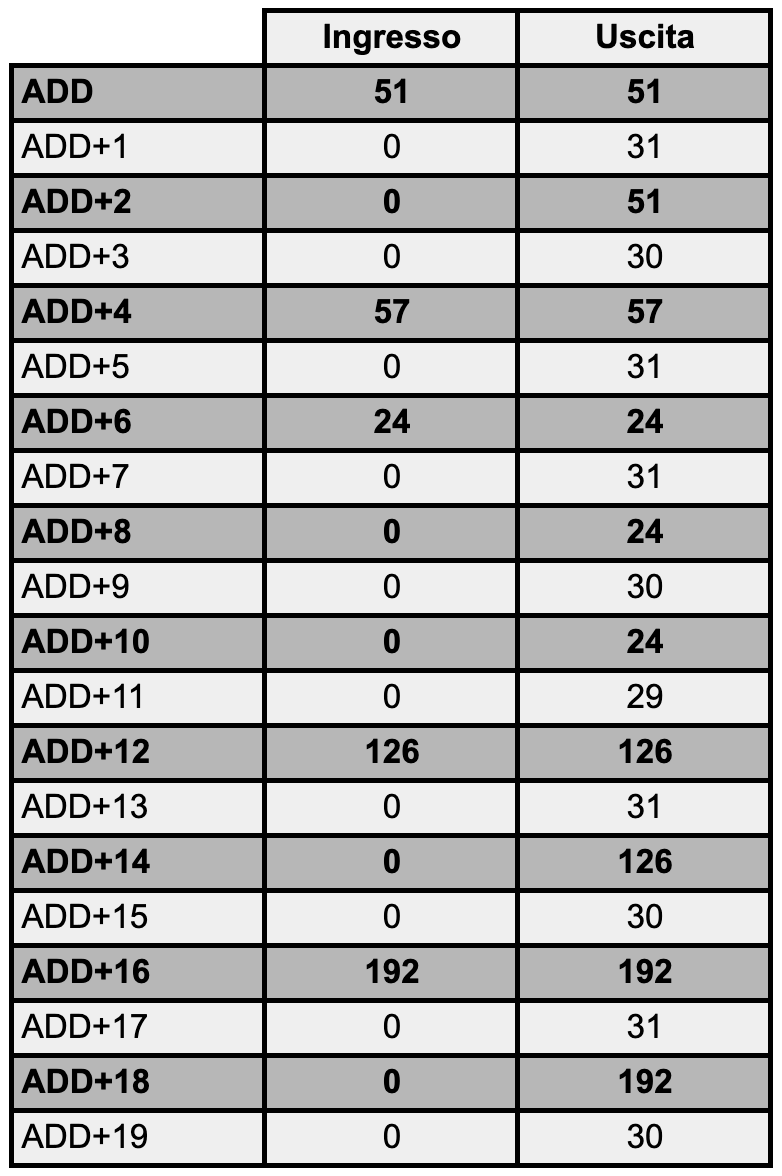
\includegraphics[width=0.45\textwidth]{figures/memory.png}
    \caption{Valori in decimale (in grassetto i valori W)}
    \label{fig:memory}
\end{figure}

\subsection{Interfaccia del componente}
Il componente descritto possiede la seguente interfaccia:

\begin{lstlisting}[basicstyle=\small, language=VHDL]
entity project_reti_logiche is
    port (
        i_clk   : in std_logic;
        i_rst   : in std_logic;
        i_start : in std_logic;
        i_add   : in std_logic_vector(15 downto 0);
        i_k     : in std_logic_vector(9 downto 0);

        o_done : out std_logic;

        o_mem_addr : out std_logic_vector(15 downto 0) ;
        i_mem_data : in std_logic_vector(7 downto 0);
        o_mem_data : out std_logic_vector(7 downto 0);
        o_mem_we   : out std_logic;
        o_mem_en   : out std_logic
) ;
end entity;
\end{lstlisting}

In particolare:
\begin{itemize}
	\item \lstinline[columns=fixed]{i_clk} è il segnale di \lstinline[columns=fixed]{CLOCK} in ingresso generato dal Test Bench;
		
	\item \lstinline[columns=fixed]{i_rst} è il segnale di \lstinline[columns=fixed]{RESET} che inizializza la macchina pronta per ricevere il primo segnale di \lstinline[columns=fixed]{START};

 	\item \lstinline[columns=fixed]{i_start} è il segnale di \lstinline[columns=fixed]{START} generato dal Test Bench;
	
	\item \lstinline[columns=fixed]{i_add} è il segnale (vettore) che indica l'indirizzo di partenza;
	
	\item \lstinline[columns=fixed]{i_k} è il segnale (vettore) che indica il numero di parole da leggere;
	
	\item \lstinline[columns=fixed]{o_done} è il segnale di uscita che comunica la fine dell'elaborazione;
	
	\item \lstinline[columns=fixed]{o_mem_addr} è il segnale (vettore) che indica l'indirizzo su cui sta lavorando la memoria;

 	\item \lstinline[columns=fixed]{i_mem_data} è il segnale (vettore) di ingresso dalla memoria al nostro componente;

  	\item \lstinline[columns=fixed]{o_mem_data} è il segnale (vettore) di uscita dal componente verso la memoria.

  	\item \lstinline[columns=fixed]{o_mem_en} è il segnale di \lstinline[columns=fixed]{ENABLE} da dover mandare alla memoria per poter comunicare (sia in lettura che in scrittura);
	
	\item \lstinline[columns=fixed]{o_mem_we} è il segnale di \lstinline[columns=fixed]{WRITE ENABLE} da dover mandare alla memoria per poterci scrivere.
\end{itemize}